
\begin{figure*}
\vspace{2mm}
\centering
    \subfigure[Max Prob. All Sets Covered vs. N (Timeliness = 50)]{
	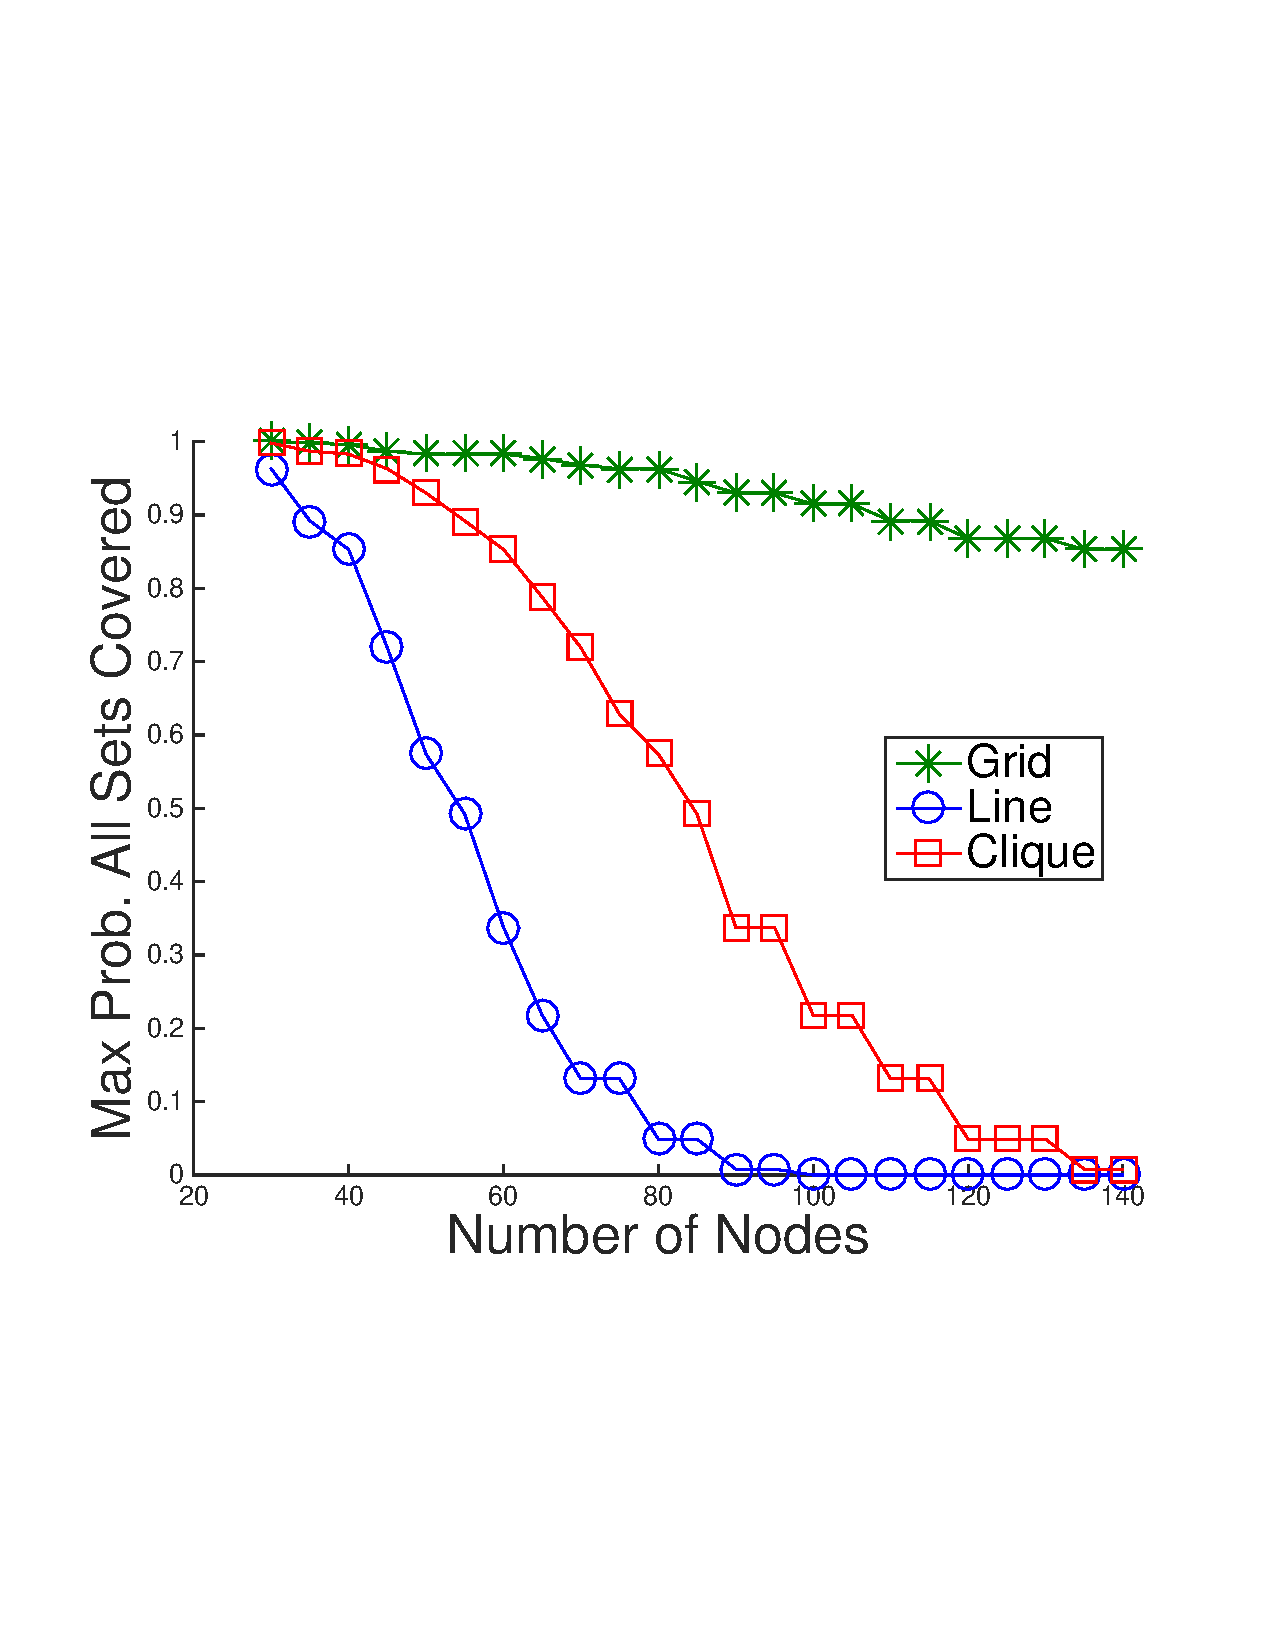
\includegraphics[scale=0.28, clip=true, trim=14mm 65mm 22mm 65mm]{figures/use_cases_examples/cluster/cluster_cov_perc_vs_num_nodes_50_T_12_IS_2_W_color.pdf}
        \label{fig:use_case_sum_sim_vs_num_nodes}
        }
  \subfigure[Max N vs. Timeliness (Prob. All Sets Covered = 0.8)]{
	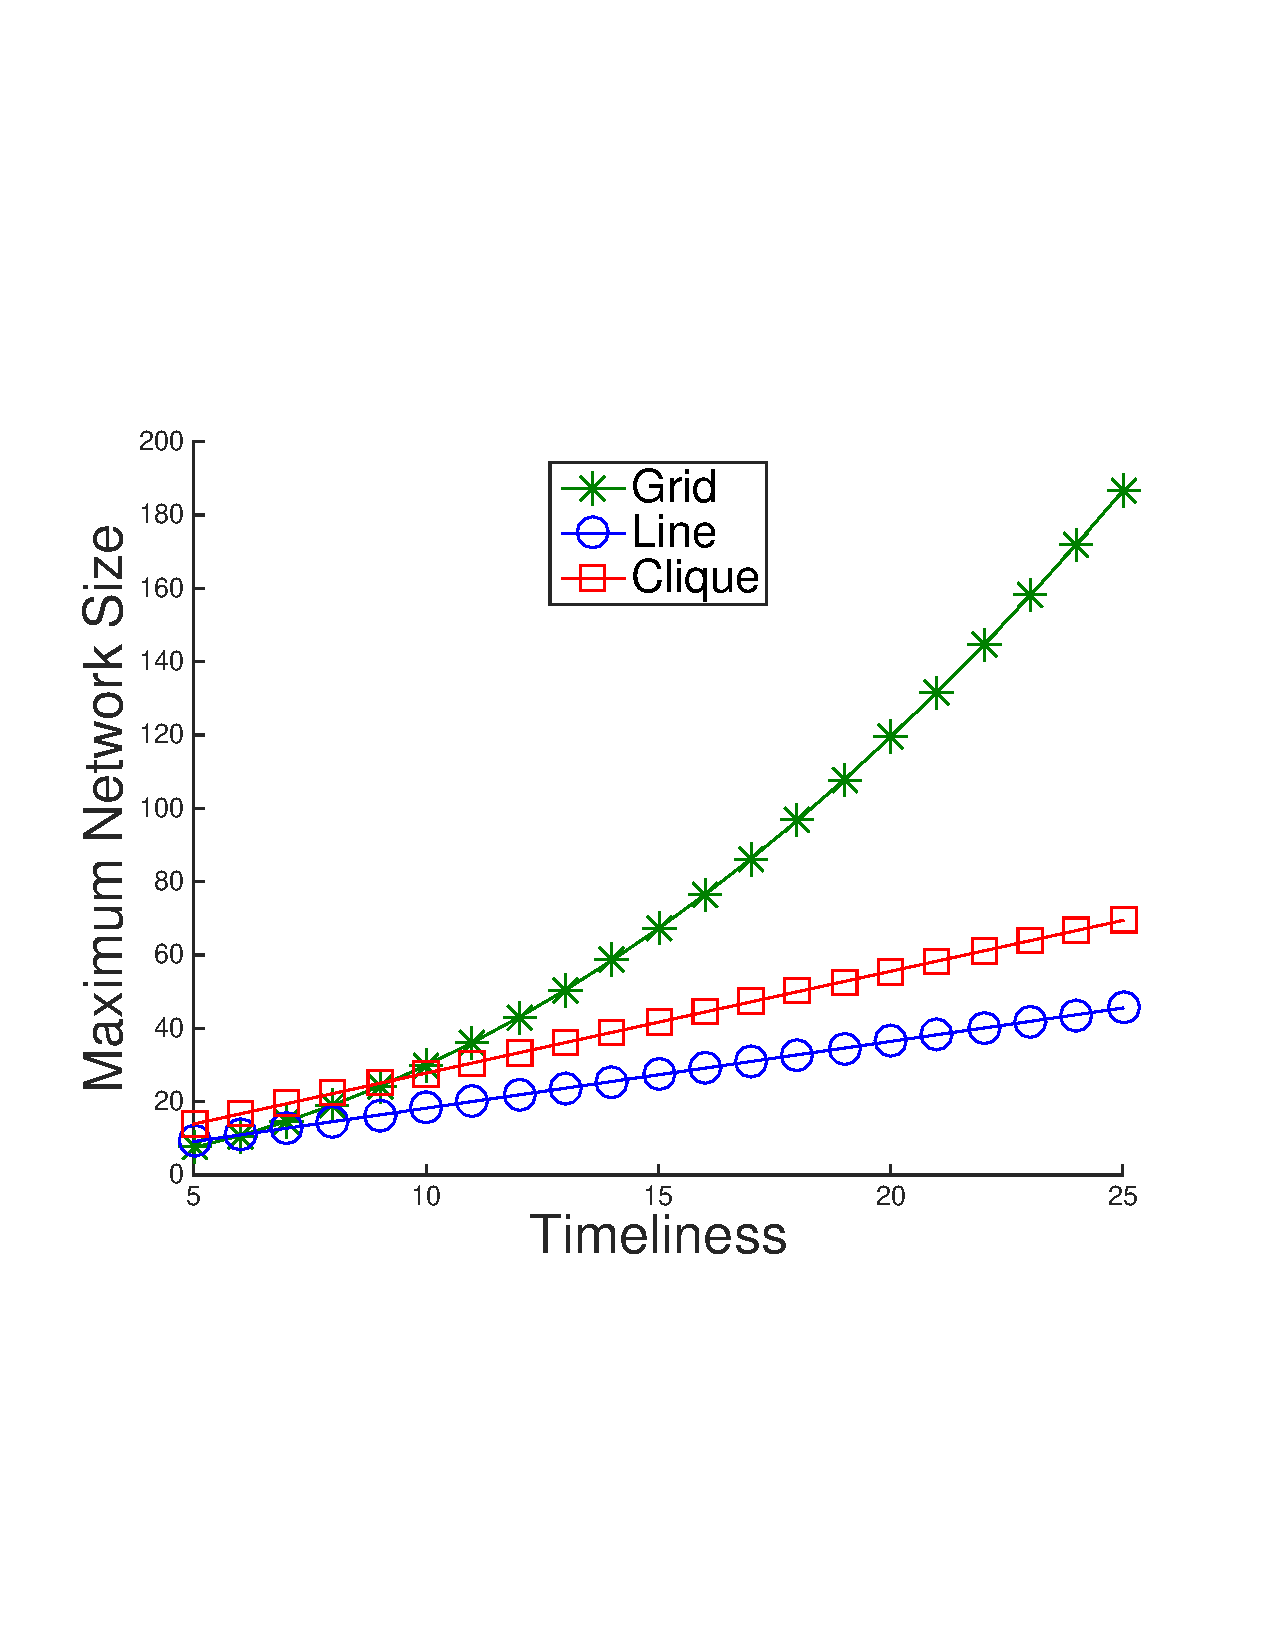
\includegraphics[scale=0.28, clip=true, trim=14mm 65mm 23mm 65mm]{figures/use_cases_examples/cluster/num_nodes_vs_tness_cluster_color.pdf}
        \label{fig:use_case_num_nodes_vs_qoi_2}
        }
  \subfigure[Max Prob. All Sets Covered vs. Timeliness (N = 14)]{
	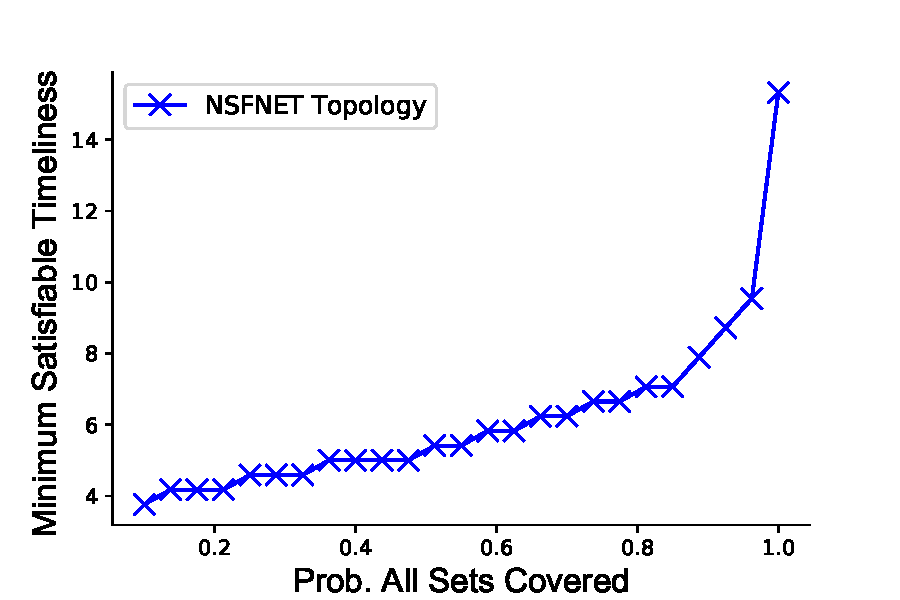
\includegraphics[scale=0.45, clip=true, trim=0mm 0mm 0mm 0mm]{figures/use_cases_examples/nsf_net/prob_sets_cov_vs_tness.pdf}
        \label{fig:use_case_nsf}
        }
   \vspace{-1mm}
   \caption{Varying design parameters provide immediate limitations as well as evident trends and comparisons. Scalability equation can be used for showing tradeoff in QoI requirements as shown here for the NSFNET topology. }
   \label{fig:huh_net_design}
   \vspace{-6mm}
\end{figure*}

\section{Impact on Network Design}
\label{sec:network_design}
Now that we have established a model for QoI satisfiability and scalability and shown its accuracy in predicting estimated limits, we show how it can also provide quick, but useful intuition about the impact of various network parameters.  Once an equation for a network's limitations is formulated as was done for equations in Table \ref{table:scal_eqs}, it can be solved for a single parameter to gain an understanding of its reliance on the other factors.  This analysis can be done very quickly and easily by approximating when appropriate, or by using symbolic and/or numerical solvers.  

%\subsection{Example Scalability and QoI Satisfiability Trends}
To exemplify this application in network design, we have applied this process to the equations in Table \ref{table:scal_eqs} using the probability that all settings of interest will be represented, or covered, by the set of images returned by the clustering algorithm explained in Section \ref{sec:qoi_model} as the completeness metric.  Recall that the highly non-linear relationship between the number of images collected and probability of covering all sets, of which there are $9$ in our experimental setup, is given in the empirical results of Figure \ref{fig:clusterAvgNumSetsCov}.  We present several figures that provide insight into network limitations and tradeoffs. 

%Figure \ref{fig:use_case_tness_vs_num_nodes} shows minimum satisfiable timeliness values for different topologies of increasing size.  While it may be intuitive that a grid network should be able to serve flows with lower timeliness constraints than a line network since it will have shorter average path lengths, what is not intuitive is \emph{how much} lower of a timeliness constraint is satisfiable.  Here, we see that a grid network can scale up to over $250$ nodes while supporting flows with $T = 50$.  A line network, on the other hand, can only scale to only approximately $20\%$ of that network size for the same timeliness value.  
%Additionally, it is useful to know how a clique network's timeliness satisfiability scales in comparison to either a grid or line network since its operation is quite different.

Figure \ref{fig:use_case_sum_sim_vs_num_nodes} visualizes the maximum expected probability that the images returned will create a complete cover of locations for a query given a fixed timeliness constraint of $T=50$ seconds. 
%As the network size increases, the probability of covering all sets decreases because the overall increase in traffic from more queries reduces the number of images each query can serve.
While it may be intuitive that a grid network's ability to deliver valuable content does not degrade as much as the line or clique network, what is not intuitive is \emph{how much} of a difference we should expect. Here, we see that as the line network becomes completely overloaded at $90$ nodes, the grid network can scale up to over $140$ nodes while supporting flows with a $90\%$ probability of delivering a complete cover.
%Here, again, limits and trends are quickly evident.  
% Again, determining the exact impact on QoI is not intuitive without a clear relationship like those given in the derived scalability equations.  In addition, the nonlinearity of completeness requirements are evident here as the data requirements for the highest completeness requirements are only sustainable for small networks, and achievable completeness diminishes quickly as the network size grows for both line and clique networks. 

If given a topology and application with predetermined requirements of $\mathbf{q}$, we may be interested in how large our network can grow before its capacity to deliver the desired QoI per flow is no longer possible. An example of an answer to this question is in Figure \ref{fig:use_case_num_nodes_vs_qoi_2}.  This graphs shows the major impact timeliness requirements can have on maximum network size.

Finally, for networks of a fixed size, we can use the scalability equations to determine limits and tradeoffs in the other parameters in the network, especially various QoI requirements. Figure \ref{fig:use_case_nsf} shows the timeliness constraints that can be satisfied for a desired probability of collecting images that cover all areas of interest. This detailed understanding of the relationship between competing QoI requirements is not only of great utility to a network designer, but would also be of use to applications looking to optimize tradeoffs without wasting precious resources while trying to learn how these parameters affect each other. 

%\subsection{Example Total Query Rate Trends}
%Since our focus is to include wireless ad hoc networks in which all nodes can request data, one further analysis can help provide insight into how the network's total traffic is scaling with respect to varying QoI requirements.  Recall from Section \ref{sec:example_applications} that each node in this model generates queries with a completeness requirement at an average rate of $\lambda$.  Therefore, the overall number of queries that the network can support is given by the maximum number of nodes, $N$, multiplied by the query rate per node, $\lamdba$.



